With the results found in this paper, we have accurately described what kind of behavior is present about the non-smooth bifurcation when new mechanisms are introduced in both the one-dimensional model \eqref{eq:oneD_canonical} and two-dimensional Stommel model \eqref{eq:twoD_canonical}. We had considered the mixture of early bifurcation due to high oscillatory forcing $\Omega\gg 1$ with amplitude $A\sim O(1)$ and the delayed tipping due to slow variation in the bifurcating parameter at rate $\epsilon$ where $\epsilon \ll 1$. The main result being that these mechanisms have opposite effects on the tipping/bifurcation and do mix with a kind of weighted average to produce an effective tipping approximation. These results give insight into the hysteresis behavior of the Stommel model and the understudied realm of non-smooth dynamics. The work presented here used asymptotic expansions as well as the methods of multiple scales to identify reduced equations and find asymptotic solutions to the systems of differential equations. We found that depending on the region and mechanism, the reduced equations have differing expressions depending on the size of the solution. We also discover that linking the slow variation $\epsilon$ and the frequency $\Omega$ gives important insight into how the system will behave. 

The method developed in the one-dimensional model was to form an outer asymptotic expansion by separating the order of dynamics by a common small value, typically in terms of $\epsilon$. With the outer dynamics found, we scaled the model to find the inner equations to typically be a simpler problem. From the inner equations, we solve and determine when the solution is no longer controllable. This results in the tipping/bifurcations in the one-dimensional system \eqref{eq:oneD_canonical} which had good agreement with the numerical results from a simple differential equation solver. Due to the many similarities to the two-dimensional system \eqref{eq:twoD_canonical} we were able to modify the same analysis to find the tipping/bifurcations here as well.

Although the work here is not entirely finished as an analysis would need to be done on cases where $\Omega\sim O(1)$ or smaller. This mechanism functions qualitatively different as slow oscillations have more contribution to the dynamics. This is also seen from the analysis where low frequency oscillations no longer allow for asymptotic expansions in terms of $\Omega^{-1}$ and no longer fall under our assumptions to integrate with $T_1$ and $T_2$. Thus this case behaves fundamentally different and can influence tipping in a way we hadn't explored here. Also, large amplitude behavior $A\gg 1$ can force an additional rescaling before any familiar approaches hold. In figure~\ref{conclusion/low_freq} we show an example of these mechanisms which shows their different influence on the system. These cases were mentioned but have yet to be performed on this model, although both have been studied around the smooth case in \cite{zhu2015tipping}. It is possible that they could have some surprising results in the non-smooth case. These cases would help further classify the tipping behavior for the variety of cases in real world ocean dynamics.

\begin{figure}[H]
\centering
\begin{subfigure}{.5\textwidth}
  \centering
  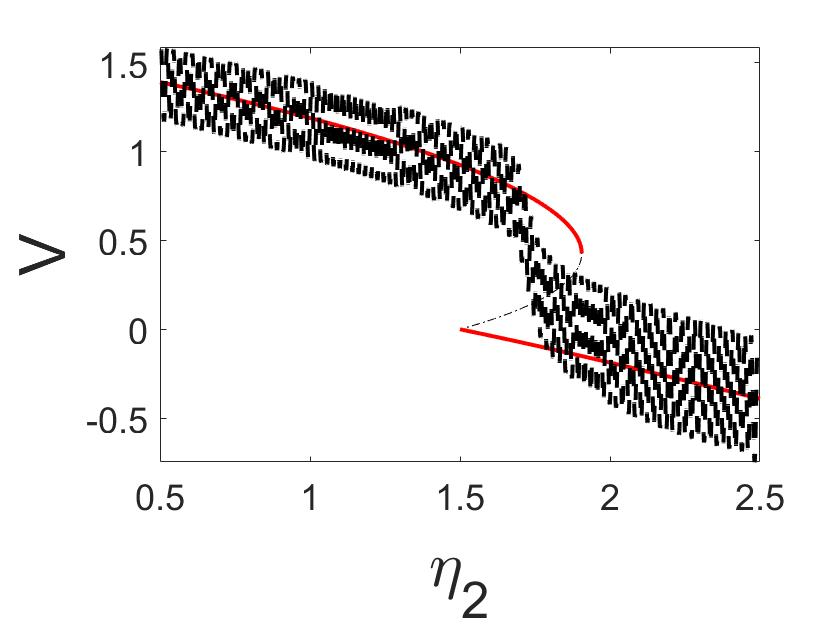
\includegraphics[width=\linewidth]{conclusion/low_freq_V.jpg}
  \caption{}
\end{subfigure}%
\begin{subfigure}{.5\textwidth}
  \centering
  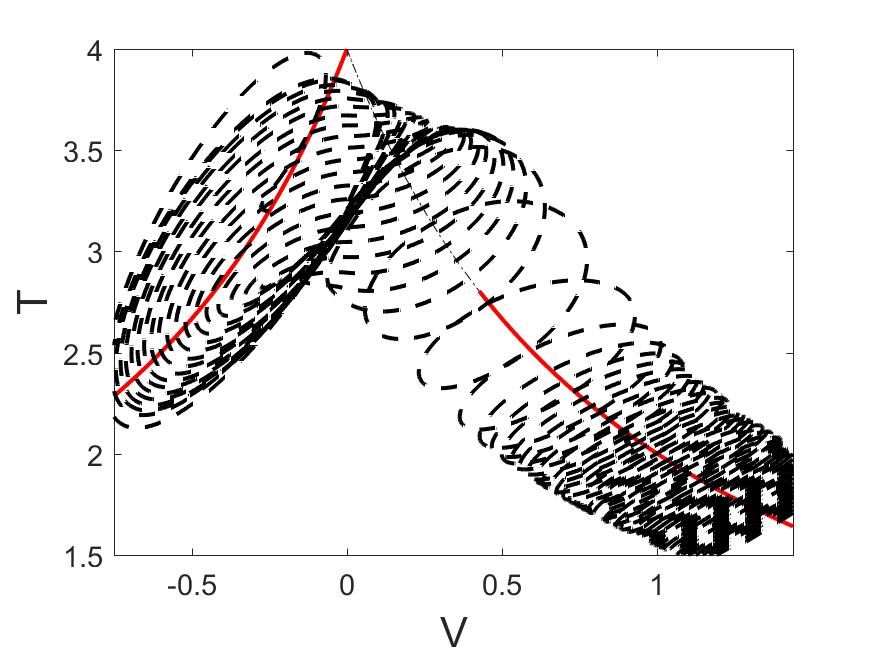
\includegraphics[width=\linewidth]{conclusion/low_freq_T.jpg}
  \caption{}
\end{subfigure}
\caption{Model parameters are $\epsilon=.01$ and $\Omega=3$.}
\label{fig:low_freq}
\end{figure}